
    \section{基于图像增强}

    \subsection{直方图均衡化}
    \begin{frame}
      \frametitle{直方图均衡化}
      直方图均衡化算法的基本思想是通过直方图均衡化来扩大原有雾图像的灰度范围,改善原有雾图像对比度低的问题。
      \begin{figure}
        \centering
        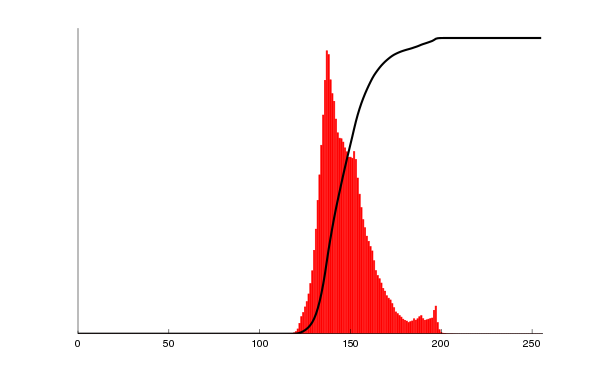
\includegraphics[width=0.47\textwidth]{figures/pic2.png}
        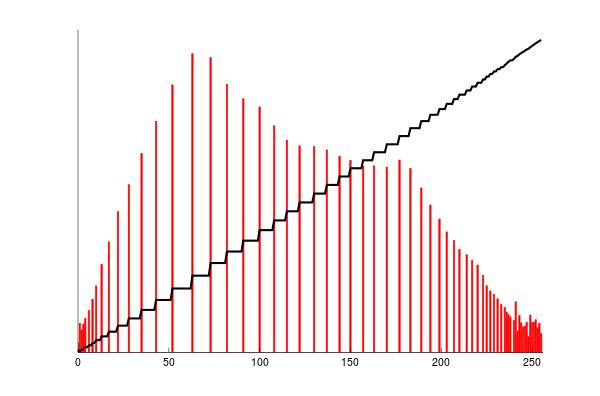
\includegraphics[width=0.45\textwidth]{figures/pic3.png}
        \caption{直方图均衡化示意图}
      \end{figure}
    \end{frame}
    \begin{frame}
      \frametitle{直方图均衡化}
      \begin{figure}
        \centering
        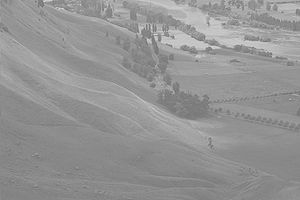
\includegraphics[width=0.45\textwidth]{figures/pic4.jpg}
        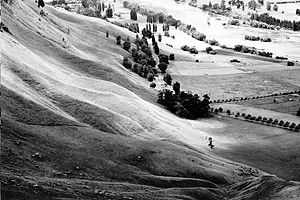
\includegraphics[width=0.45\textwidth]{figures/pic5.jpg}
        \caption{直方图均衡化效果图}
      \end{figure}
    \end{frame}


    \subsection{同态滤波}
    \begin{frame}
      \frametitle{同态滤波}
      同态滤波是一种在频域内对图像进行对比度增强的算法。同态滤波算法将有雾图像的复原问题转换成增大有雾图像频域范围的问题,通过减少有雾图像中的低频信息,并相应增加图像中的高频信息,可以实现图像去雾的效果。
      \begin{figure}%插入一张图片
        \centering
        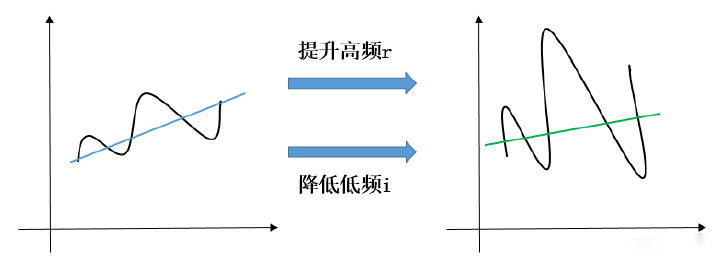
\includegraphics[width=\textwidth]{figures/pic6.png}
        \caption{同态滤波示意图}
      \end{figure}
    \end{frame}

    \begin{frame}
      \begin{equation}
        f(x,y)=i(x,y)·r(x,y)
      \end{equation}

      \begin{equation}
        z(x,y)=\ln f(x,y) =\ln i(x,y) +\ln r(x,y)
      \end{equation}

      \begin{equation}
        Z(u,v)=Fi(u,v) +Fr(u,v)
      \end{equation}

      \begin{equation}
        S(u,v)=H(u,v)S(u,v)=H(u,v)·Fi(u,v) +H(u,v)·Fr(u,v)
      \end{equation}

      \begin{equation}
        s(u,v)=IDFT(S(u,v))
      \end{equation}

      \begin{equation}
        g(x,y)=e^{s(x,y)}=io(x,y)·ro(x,y)
      \end{equation}
    \end{frame}


    \begin{frame}
      \frametitle{同态滤波}
      \begin{figure}%插入一张图片
        \centering
        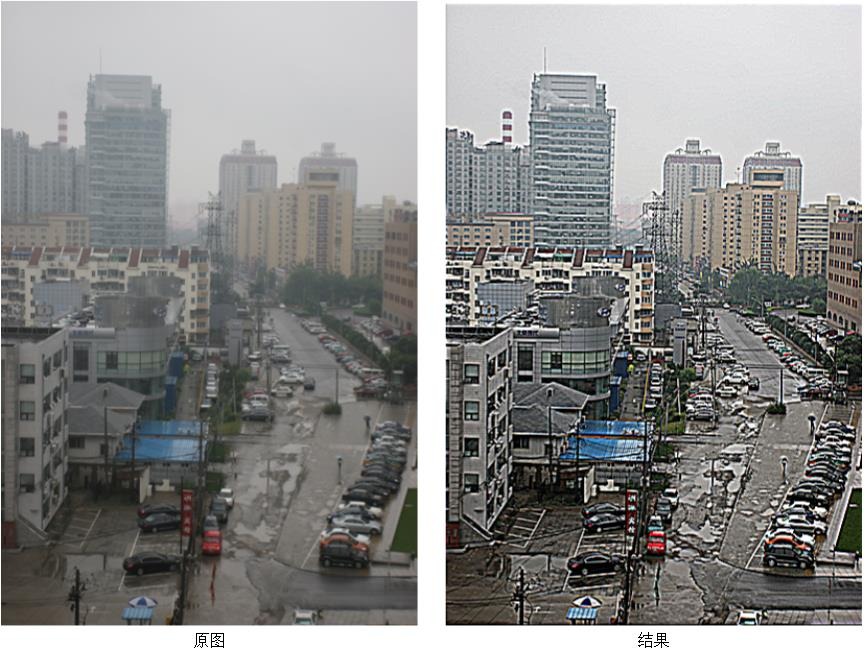
\includegraphics[width=0.8\textwidth]{figures/pic7.png}
        \caption{同态滤波效果图}
      \end{figure}
    \end{frame}


    \subsection{Retinex算法}
    \begin{frame}
      \frametitle{Retinex算法}
      Retinex算法是一种基于人类视觉系统的图像增强算法,它通过对图像进行多尺度分解,然后对每个尺度的图像进行对比度增强,最后将所有尺度的图像进行融合,从而实现图像增强的目的。

      \centering
      %斜体字
      \textit{Retinex~=~retina(视网膜)~+~cortex(皮层)}

    \end{frame}

    \begin{frame}
      \frametitle{Retinex算法}
      \begin{itemize}
        \item 1.将一幅有雾图像$S(x,y)$表示成反射分量$R(x,y)$和亮度分量$L(x,y)$的乘积形式:
          \begin{equation}
            S(x,y)=R(x,y)·L(x,y)
          \end{equation}
        \item 2.对第一步中的式两边分别取对数并移项,结果如下:
          \begin{equation}
            \ln(R(x,y))=\ln(S(x,y))-\ln(L(x,y))
          \end{equation}
      \end{itemize}
    \end{frame}

    \begin{frame}
      \frametitle{Retinex算法}
      \begin{itemize}
        \item 3.对上式去除亮度分量$L(x, y)$,求得反射分量 $R(u, v)$,从而得到增强后的图像,实现原图像的去雾处理。
        \begin{equation}
              L(x,y)=S(x,y)*H(x,y)
        \end{equation}
        \begin{equation}
              H(x,y)=u·exp(-\frac{x^2+y^2}{\sigma^2})
        \end{equation}

        $*$为卷积操作,$u$为归一化值,$\sigma$为高斯环绕尺度参数。
        \begin{equation}
           \ln(R_c(x,y))=\ln(S_c(x,y))-\ln(S_c(x,y) * H(x,y))
        \end{equation}

        $c$表示彩色图像RGB颜色空间中的某一颜色通道。

      \end{itemize}
    \end{frame}

